\section{Results}
\subsection{Unitary Gates}
Translating Pulser's native unitary gate to QASM's unitary gate was only partially successful. Three of the four comparisons made on each test iteration were successful.
the eigenvalues for the $|0 \rangle$ are equal, however the eigenvalues of the $|1 \rangle$ state is in the wrong phase.
\begin{wrapfigure}{l}{65mm}
    \centering
    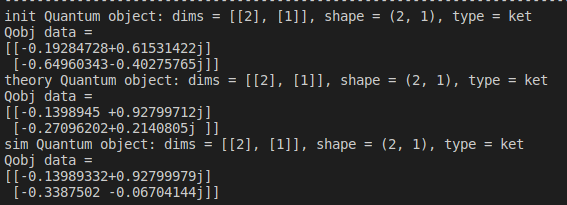
\includegraphics[width=65mm]{./Images/QASM_U_result.png}
    \caption{Example resulting states of A QASM\_U test} 
    \label{fig:[QASM_U]}
  
  \end{wrapfigure}
As seen in the figure, the eigenvalues for the $|0 \rangle$ are identical up to an accuracy of $10^{-5}$, but the $|1 \rangle$ states are different.
However, if the absolute value is taken:\\
- $\sqrt(-0.27096202^{2}+0.2140805^{2}) = 0.34532720246$ \\
- $\sqrt(-0.3387502^{2}+0.06704144^{2}) = 0.34532050717$\\
\\\\\\
We notice that the measurement probabilities are indeed correct, thus there is a phase issue around the $|1 \rangle$ state.


\subsection{Pauli and Hadammard Gates}
Similar to the QASM unitary gates the implementation of Pauli gates suffers phase issues.
The phase issues result in a sign flip either on the $|0 \rangle$ state or the $|1 \rangle$ depending on which gate is used.
As seen in figure \ref{fig:HXYZ}, the Pauli gates flip the sign of the $|0 \rangle$ state whereas the Hadamard gate flips the sign on the $|1 \rangle$ state
\begin{figure}[H]
    \centering
    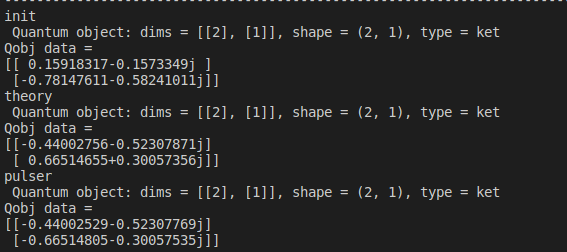
\includegraphics[width=80mm]{Images/H.png}\hfill
    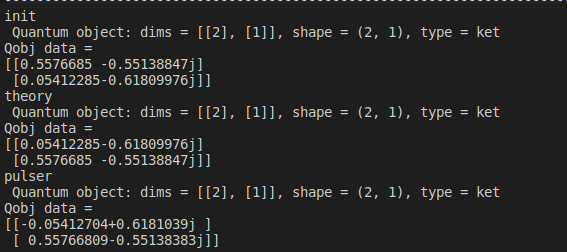
\includegraphics[width=80mm]{Images/X.png}\hfill
    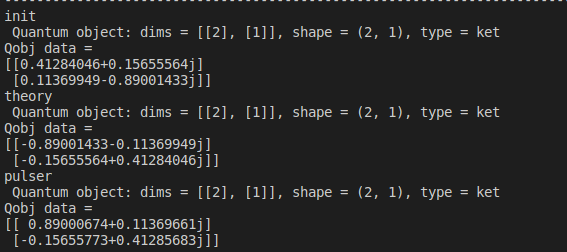
\includegraphics[width=80mm]{Images/Y.png}\hfill
    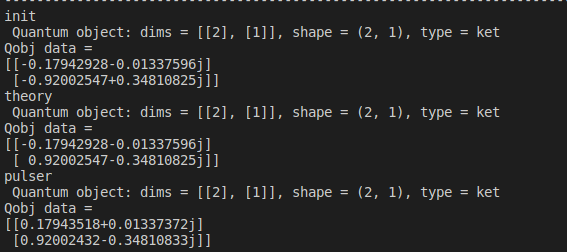
\includegraphics[width=80mm]{Images/Z.png}\hfill

    \caption{From top-left to bottom-right, an example of the Hadamard, X, Y and Z gates test results}
    \label{fig:HXYZ}
\end{figure}


\subsection{Arbitrary Rotation Gates}

\begin{figure}[H]
    \centering
    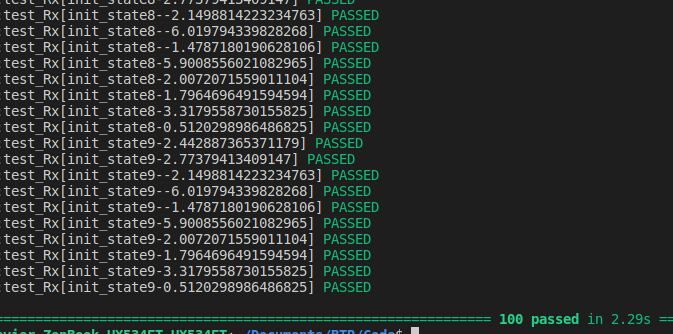
\includegraphics[width=80mm]{Images/Rx.png}\hfill
    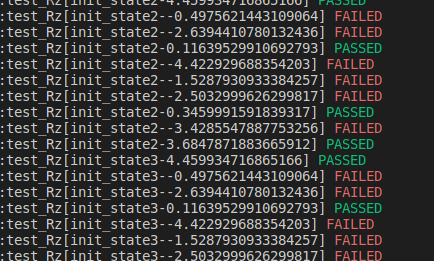
\includegraphics[width=80mm]{Images/Rz.png}
    \caption{Rx and Rz test results for 10 random initial states paired with 10 random values of $\theta \in [-2\pi, 2\pi]$}
    \label{fig:RX}
\end{figure}
 \textcolor{white}{h} \\
As mentioned in the introduction, the Rx and Ry gates can be implemented relatively easily using, Pulser's unitary gate.
For both these gates not only was the testing fully successful, but the gate fidelity was also increased to $10^{-5}$.
The Rz gate is also fully functional as long as $\theta$ remains positive. This is due to the fact Rz is implemented as a virtual gate. The phase shifts
pulser implements are always $\lambda \in [0, 2\pi]$ rather than $\lambda \in [-2\pi, 2\pi]$, thus the extra phase shift is not applied correctly when negative.


\subsection{CNOT gate}
Having been implemented, by combing two H gates and a CZ gate (H CZ H), the CNOT gate is a good way to test whether consecutive gates work correctly, but also
makes use of basis changes, since H is a single qubit gate. This allows us to test whether switching from qubits to qutrits and back works correctly.
Like the Rx and Ry gates the CNOT gate was a complete success, regardless of which qubit was designated as control, with a fidelity of $10^{-5}$. 

\begin{figure}[H]
    \centering
    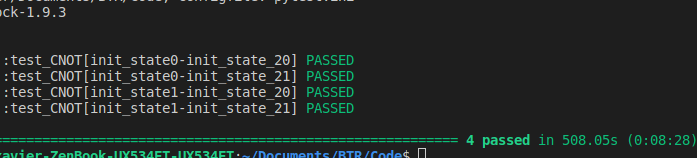
\includegraphics[width=150mm]{Images/CNOT.png}\hfill
    \caption{CNOT test results using two different random initial states}
    \label{fig:CNOT}
\end{figure}
 \textcolor{white}{h}


\newpage

\subsection{Rydberg Blockade Testing}
\begin{wrapfigure}{l}{65mm}

    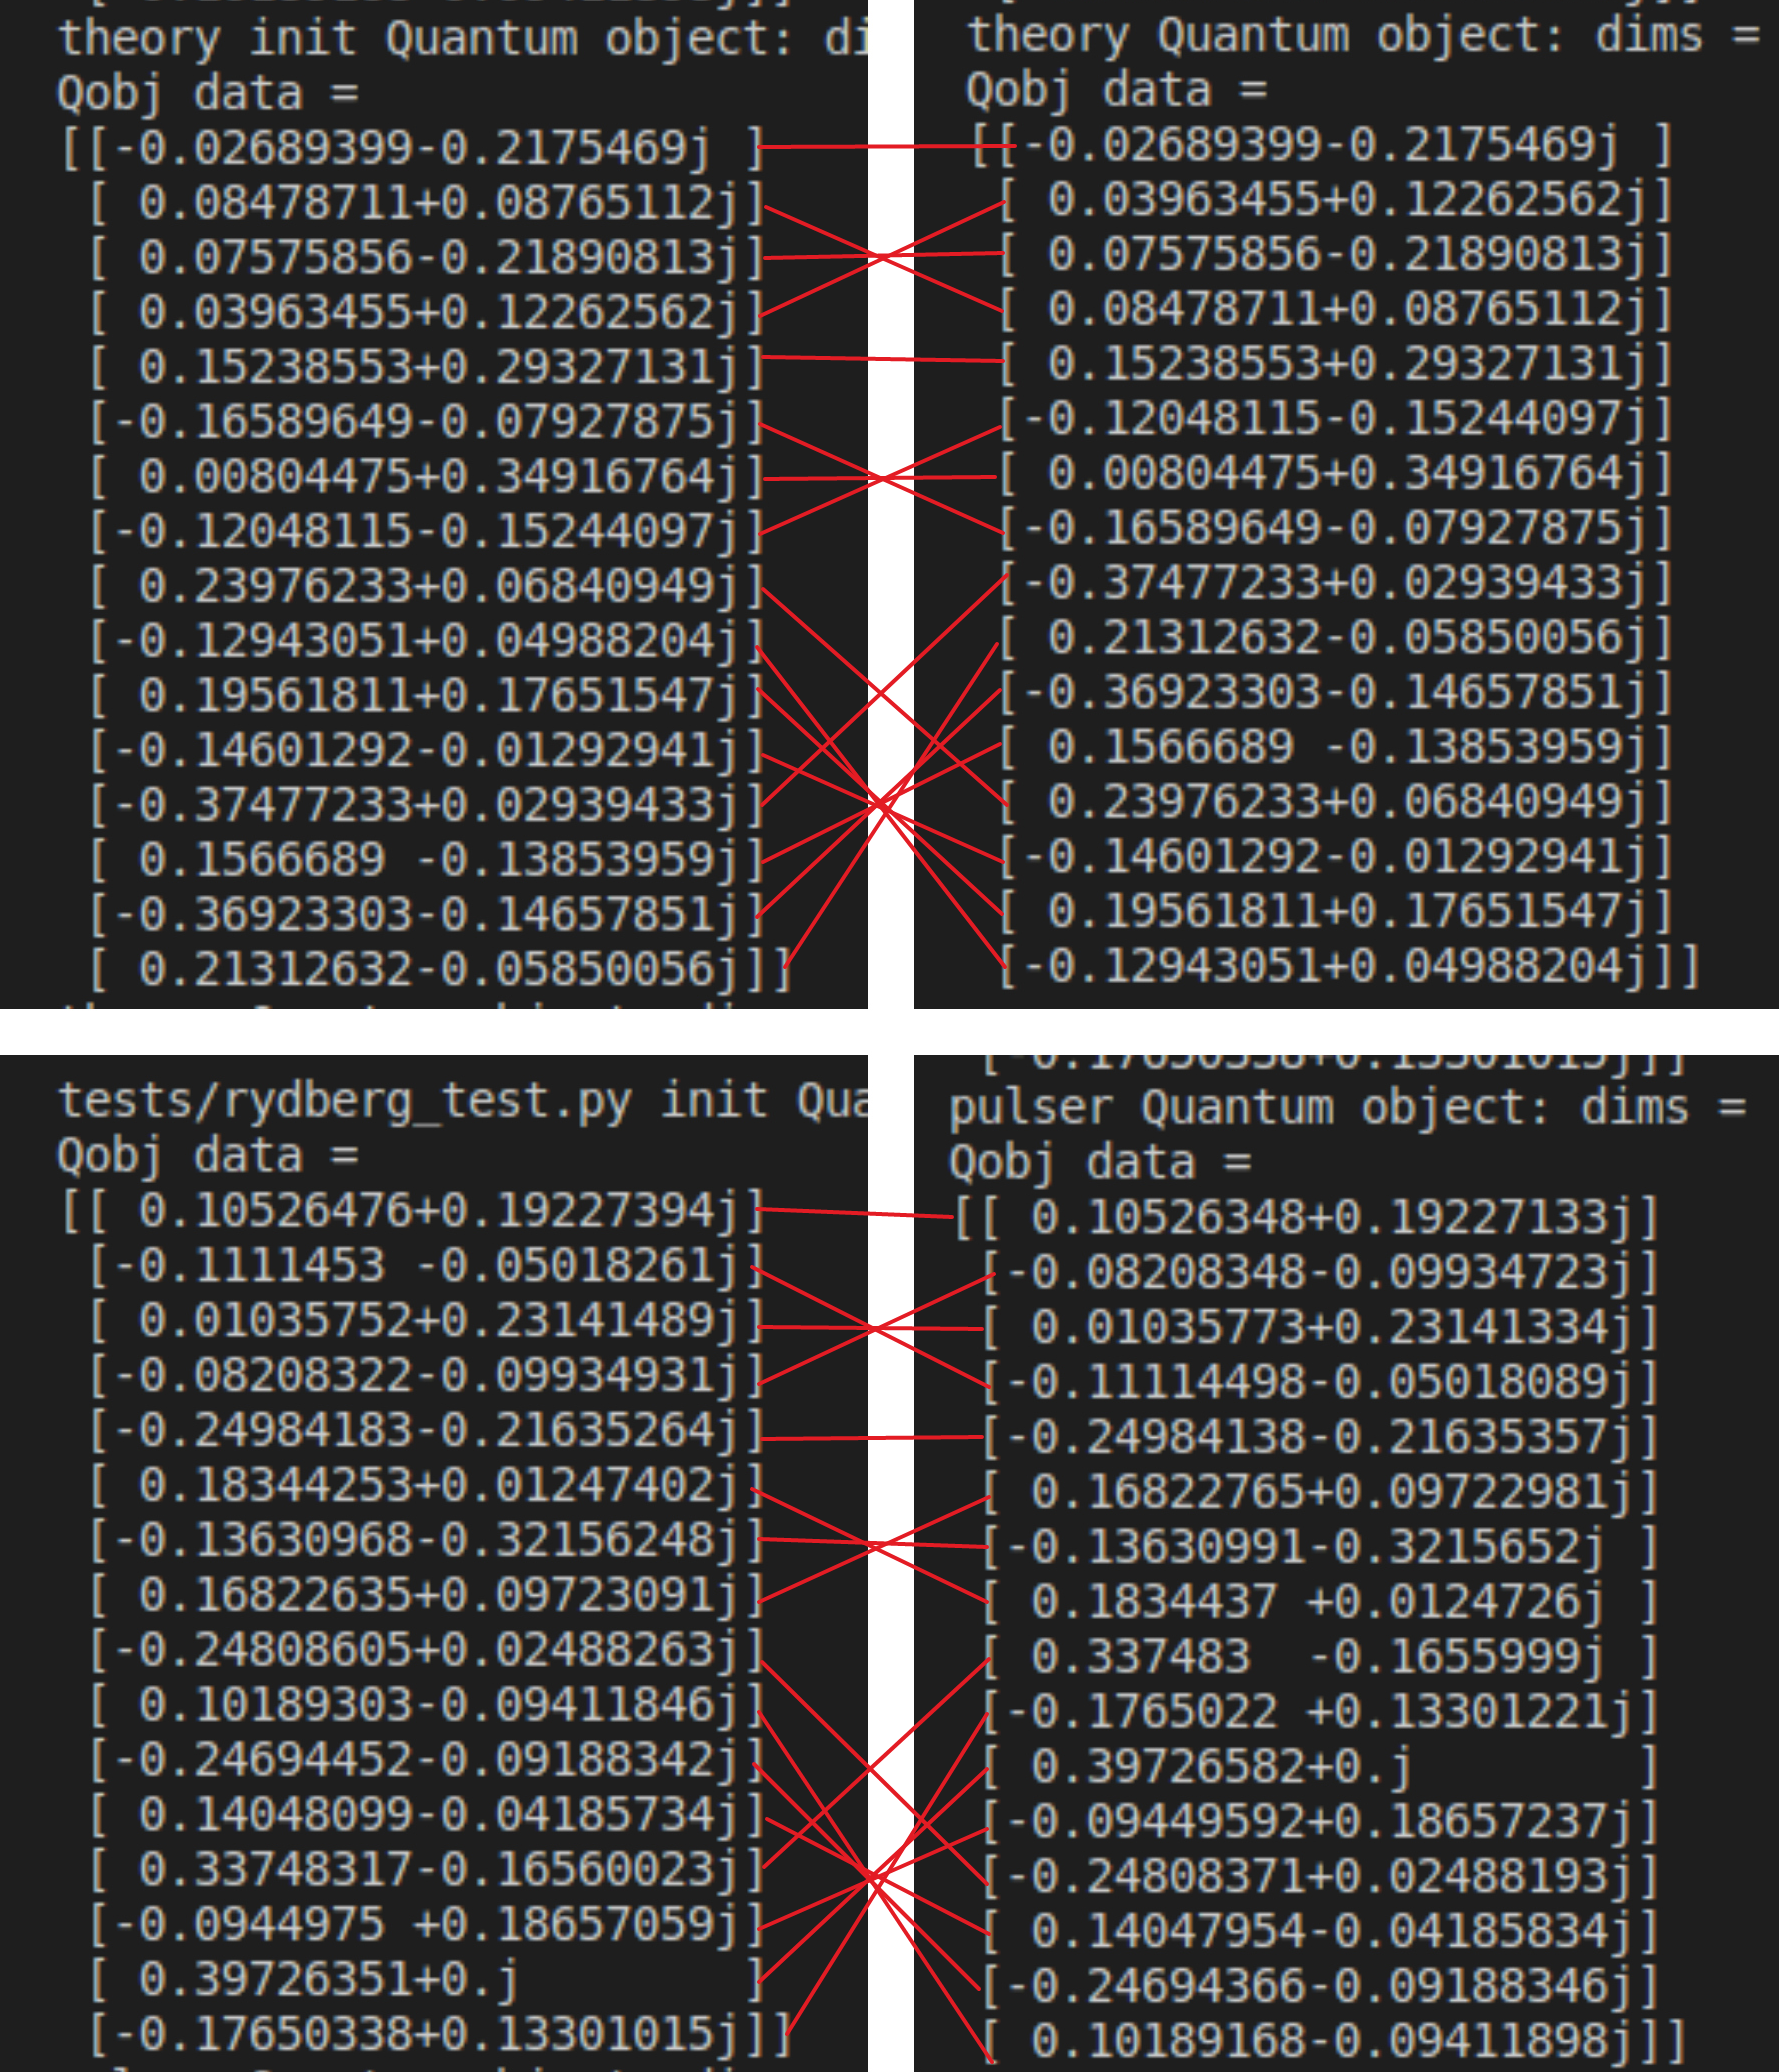
\includegraphics[width=65mm]{./Images/rydbergtest.png}
    \caption{Rydberg Blockade test results} 
    \label{fig:rydbergtest}
  
\end{wrapfigure}
\textcolor{white}{h}\\
Due to problems with changing bases from qutrits to qubits, the initial state for the theoretical gates and the Pulser simulation does not start with the same initial state.
This problem was not solved during the time of the project and thus this test cannot be considered rigorous.
However, there is some information that can be taken away, as seen in Figure 9, even though the initial states are different,
there is an obvious pattern as to how both the theoretical gate and the Pulser simulation, modify the initial state.
Both these patterns being identical, one could assume that the gate works correctly.\\\\\\\\\\





\subsection{Parsing}
While the parsing methods are far from being completed, they are already partially functional and information about the registers, defined gates and used gates can be obtained.
For the moment these methods still offer minimal syntax error detection. For example, the code is currently able to detect when the targets and controls of a two-qubit gate are badly set.
This can be illustrated in Figure 10.
\begin{lstlisting}
    gate x a { U(pi, 0, pi) a; }
    gate y a { U(pi, pi/2, pi/2) a; 
            U(pi, pi/2, pi/2) a;
    }
    
    qubit[2] q;
    qubit[3] b;
    
    cnot b, q;
    x q[1];
\end{lstlisting}

\begin{figure}[H]
    \centering
    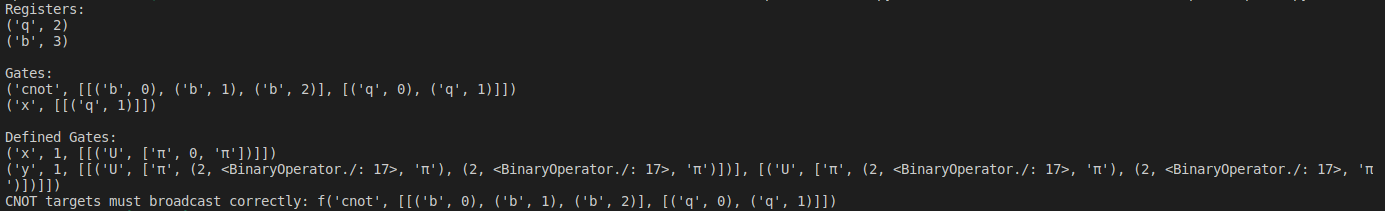
\includegraphics[width=180mm]{Images/parsing.png}\hfill
    \caption{parsing results}
    \label{fig:parsers}
\end{figure}
 \textcolor{white}{h}
